\documentclass[11pt, a4paper]{article}

\usepackage[utf8]{inputenc}
\usepackage[french]{babel}
\usepackage[T1]{fontenc}
\usepackage{verbatim}
\usepackage{color}
\usepackage{listings}
\usepackage{graphicx}
\usepackage{hyperref}
\usepackage[left=1in, right=1in, top=1in, bottom=1in]{geometry}


% $1 : fichier source
% $2 : langage
\newcommand{\addCode}[2]{%

  % Configuration de la coloration syntaxique du code
  \definecolor{colKeys}{rgb}{0,0,1}
  \definecolor{colIdentifier}{rgb}{0,0,0}
  \definecolor{colComments}{rgb}{0,0.5,1}
  \definecolor{colString}{rgb}{0.6,0.1,0.1}

  % Configuration des options 
  \lstset{%
    language = #2,%
    identifierstyle=\color{colIdentifier},%
    basicstyle=\ttfamily\scriptsize, %
    keywordstyle=\color{colKeys},%
    stringstyle=\color{colString},%
    commentstyle=\color{colComments},%
    columns = flexible,%
    %tabsize = 8,%
    showspaces = false,%
    numbers = left, numberstyle=\tiny,%
    frame = single,frameround=tttt,%
    breaklines = true, breakautoindent = true,%
    captionpos = b,%
    xrightmargin=10mm, xleftmargin = 15mm, framexleftmargin = 7mm,%
  }%
    \begin{center}
    \lstinputlisting{#1}
    \end{center}
}

\newcommand{\kw}[1]{\texttt{#1}}

\newcommand{\fontptitle}[1]{%
    {\huge{\texttt{\textbf{#1}}}}
}

\newlength{\largeurtitre}
\newlength{\largeurligne}
\newcommand{\lignedroite}[1]{%
    \setlength{\largeurtitre}{0pt}
    \setlength{\largeurligne}{0pt}
    \settowidth{\largeurtitre}{\fontptitle{#1}}
    \addtolength{\largeurligne}{\textwidth}
    \addtolength{\largeurligne}{-\largeurtitre}
    \addtolength{\largeurligne}{-4pt}
    \bigskip
    #1 \raisebox{0.3em}{\vrule depth 0pt height 0.2ex width \largeurligne}
}


\newcommand{\DescFonction}[4]{%
	\begin{minipage}{\textwidth}
	\lignedroite{\fontptitle{#1}}
	\nopagebreak[4]
	\textbf{\large{Synopsis}} \\
	\texttt{#2} \\
	\textbf{\large{Description}} \\
	#3 \\
	\textbf{\large{Valeur de retour}} \\
	#4 
	\vspace{1cm}
	\end{minipage}
}


\newcommand{\Test}[3]
{%
	\addtocounter{testno}{1}
	\begin{minipage}{\linewidth}
	\lignedroite{\textbf{\large{\kw{Test \thetestno}~-- #1}}}\\
	\textbf{\large{Description}}\\
	#2 \\
	\textbf{\large{Resultat attendu}}\\
	#3 
	\end{minipage}
	\vspace{1cm}
}

\title{Spécification des fonctions d'un pilote de périphérique de type capteur}
\author{Paul \textsc{Adenot} \and \'{E}tienne \textsc{Brodu}}
\date{}

\setlength{\parindent}{0cm}

\begin{document}
\maketitle
\tableofcontents
\newcounter{testno}

\newpage

\section{Documentation de l'API}
\DescFonction{open}
{int open(const char* filename, int flags, int perms)}
{Ouvre le capteur désigné par \kw{filename}, et renvoie un descripteur de
fichier (\emph{file descriptor}), qui l'identifie au sein du programme. 
\kw{flags} indique le mode d'ouverture, et doit être fixé à \kw{O\_RDONLY},
les capteurs étants en lecture seule. D'autres valeurs, possiblement passées
par l'utilisteur, provoque une erreur, et errno est fixé à \kw{EARG}.
L'argument \kw{perms} dénote les permission qui seront utilisée sur le fichier.
Plusieurs capteurs peuvent être ouvert 
au sein du même programme. Si un même capteur est ouvert plusieurs fois au
sein du même programme, alors plusieurs descripteurs de fichiers seront
disponibles pour lire sur un même capteur. Si le fichier précisé dans le 
premier paramêtre (\kw{filename}) n'existe pas, l'appel échoue, et \kw{open}
retourne immédiatement, avec la valeur -1.}
{Si l'appel reussi, un descripteur de fichier (entier positif). Sinon, 
-1, et \kw{errno} est fixé à l'une des valeurs suivantes :
\begin{description}
	\item[\kw{EARG} : ] L'appel a été effectué avec de mauvais arguments,
			avec une valeur autre que \kw{O\_RDONLY} pour \kw{flags}.
	\item[\kw{ENEXIST} : ] Premier argument invalide, le fichier n'existe pas.
	\item[\kw{EALREADYOPENED} :] Le périphérique est déjà ouvert.
\end{description}
}

\DescFonction{creat}
{int creat(const char *pathname, int mode);}
{Le comportement de cette fonction est similaire à celui de la fonction \kw{open}}
{Les valeurs de retours sont les mêmes que celles de la fonction \kw{open}.}

\DescFonction{close}
{int close(int fd);}
{Ferme le capteur désigné par le descripteur de fichier \kw{fd}. Celui-ci ne sera plus utilisable dans le programme.
Si le paramêtre \kw{fd} est invalide (i.e. négatif ou ne correspondant pas à un descripteur de fichier valide), \kw{close} retourne -1, et \kw{errno} est positionné à \kw{EARG}.\\
Si le capteur est en cours d'utilisation, l'appel échoue en renvoyant -1, et \kw{errno} est positionné à \kw{ECPTBUSY}.}
{Si l'appel réussi, 0 est renvoyé, -1 sinon, et \kw{errno} est positionné aux valeurs suivantes :
\begin{description}
	\item[\kw{EARG} : ] L'appel a été effectué avec de mauvais arguments, le \kw{fd} spécifié est invalide.
	\item[\kw{ECPTBUSY} : ] Le capteur est en cours d'utilisation.
\end{description}
}

\DescFonction{remove}
{int remove(const char *pathname);}
{Ferme le capteur désigné par \kw{pathname}. Il ne sera plus utilisable au sein du programme.
Si \kw{pathname} est invalide (le fichier n'existe pas, ou n'est pas ouvert au sein du programme), alors l'appel échoue en renvoyant -1, et \kw{errno} est positionné ) \kw{ENEXIST}.
Si le capteur est en cours d'utilisation, l'appel échoue en renvoyant -1, et \kw{errno} est positionné à \kw{ECPTBUSY}.}
{Si l'appel réussi, 0 est renvoyé, -1 sinon, \kw{errno} est positionné à l'une des valeurs suivantes :
\begin{description}
	\item[\kw{EARG} : ] Le fichier précisé n'existe pas.
	\item[\kw{ECPTBUSY} : ] Le capteur est en cours d'utilisation.
\end{description}
}

\DescFonction{read}
{int read (int fd, char *buffer, size\_t maxbytes);}
{Lit un message d'un capteur désigné par \kw{fd}, et le place dans l'adresse pointé par \kw{buffer}.
Si un message est disponible, alors il est placé dans à l'adresse \kw{buffer}, mais n'est pas \emph{consommé}, la lecture étant non destructive.
Un message lu sur un capteur est du type \kw{capt\_msg}, qui est défini de la manière suivante :
\addCode{ressources/code.c}{c}
L'entier \kw{ID} est commun à tous les capteurs, et est incrémenté à chaque message. Lors de l'initialisation du driver, il est fixé à zéro. En cas de dépassement de capacité, la valeur de \kw{ID} redeviendra 0, et continuera normalement.

La date \kw{date} est un entier, qui correspond au nombre de périodes de 20ms qui se sont écoulés depuis le démarrage du système. Il sert donc à ordonner temporellement les message, et non à déterminer leur date d'arrivée.}
{Un entier positif, correspondant à la taille lue (\kw{TAILLE\_MSG}) est renvoyée. En cas d'erreur, -1 est renvoyé, et \kw{errno} est positionné aux valeurs suivantes :
\begin{description}
	\item[\kw{EARG} : ] L'appel a été effectué avec de mauvais arguments.
	\item[\kw{ENOAVAIL} : ] Aucun message n'est disponible.
\end{description}
}

\DescFonction{write}
{int write (int fd, char *buffer, size\_t maxbytes);}
{Appel non supporté, les capteurs sont en lecture seule. Pour faire une
opération sur un capteur en fonctionnement, utiliser \kw{ioctl}.}
{N.A.}
	
\DescFonction{ioctl}
{int ioctl(int fd, int request, int value);}
{Configuration du pilote. Le paramètre \kw{request} doit être égal à la
constant \kw{CHANGEMENT\_CAPTEUR}. La valeur de \kw{value} doit alors être
inférieur ou égale à 255, et correspond au nouveau numéro de capteur
pour le descripteur de fichier passé en premier argument.}
{\kw{ioctl} renvoie 0 en cas de succès, -1 sinon, et \kw{errno} est alors positionné à l'une des valeurs suivantes :
\begin{description}
	\item[\kw{EARG} : ] L'appel a été effectué avec de mauvais arguments.
	\item[\kw{ECPTBUSY} : ] Le capteur est occupé, il doit être possible de
	recommencer l'appel avec succès dans un futur proche.
\end{description}
}

\section{Structure des données}

\subsection{table\_capteur}
Ce tableau contient les descripteur de chaque capteur créé.

Structures décrivant un capteur :
\addCode{ressources/descr_capt.c}{c}

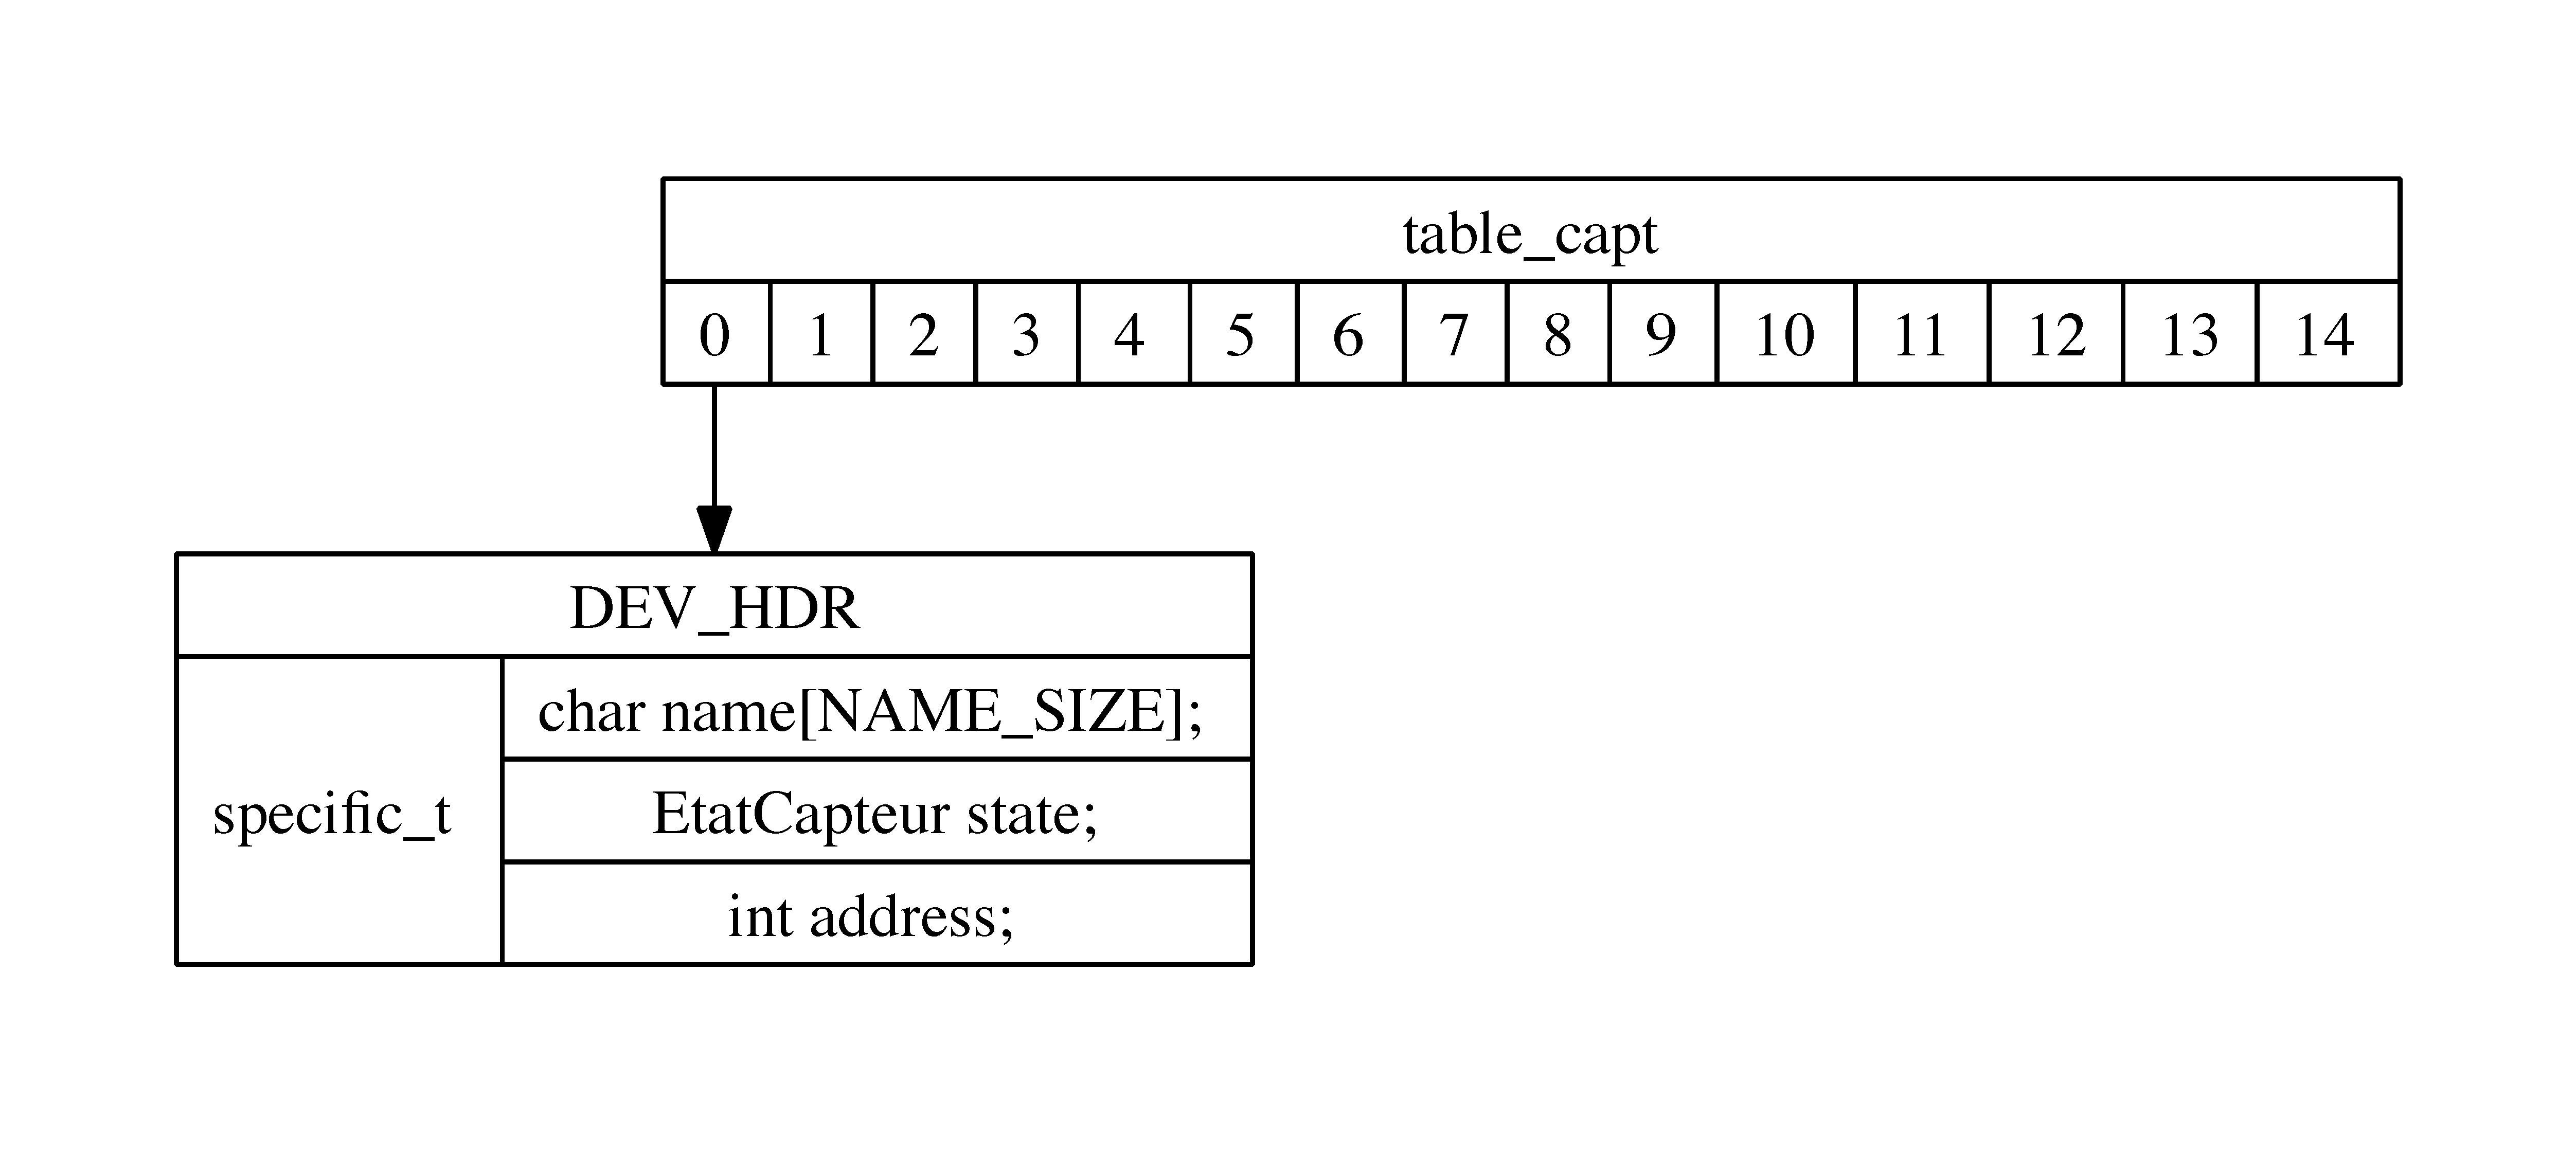
\includegraphics[width=\textwidth]{ressources/table_capteur.pdf}\\

\subsection{table\_buffer}
Ce tableau contient à l'index $i$ le dernier message du périphérique \kw{/dev/capteur}$i$ créé à la position $i$ dans \kw{tableau\_capteur}.

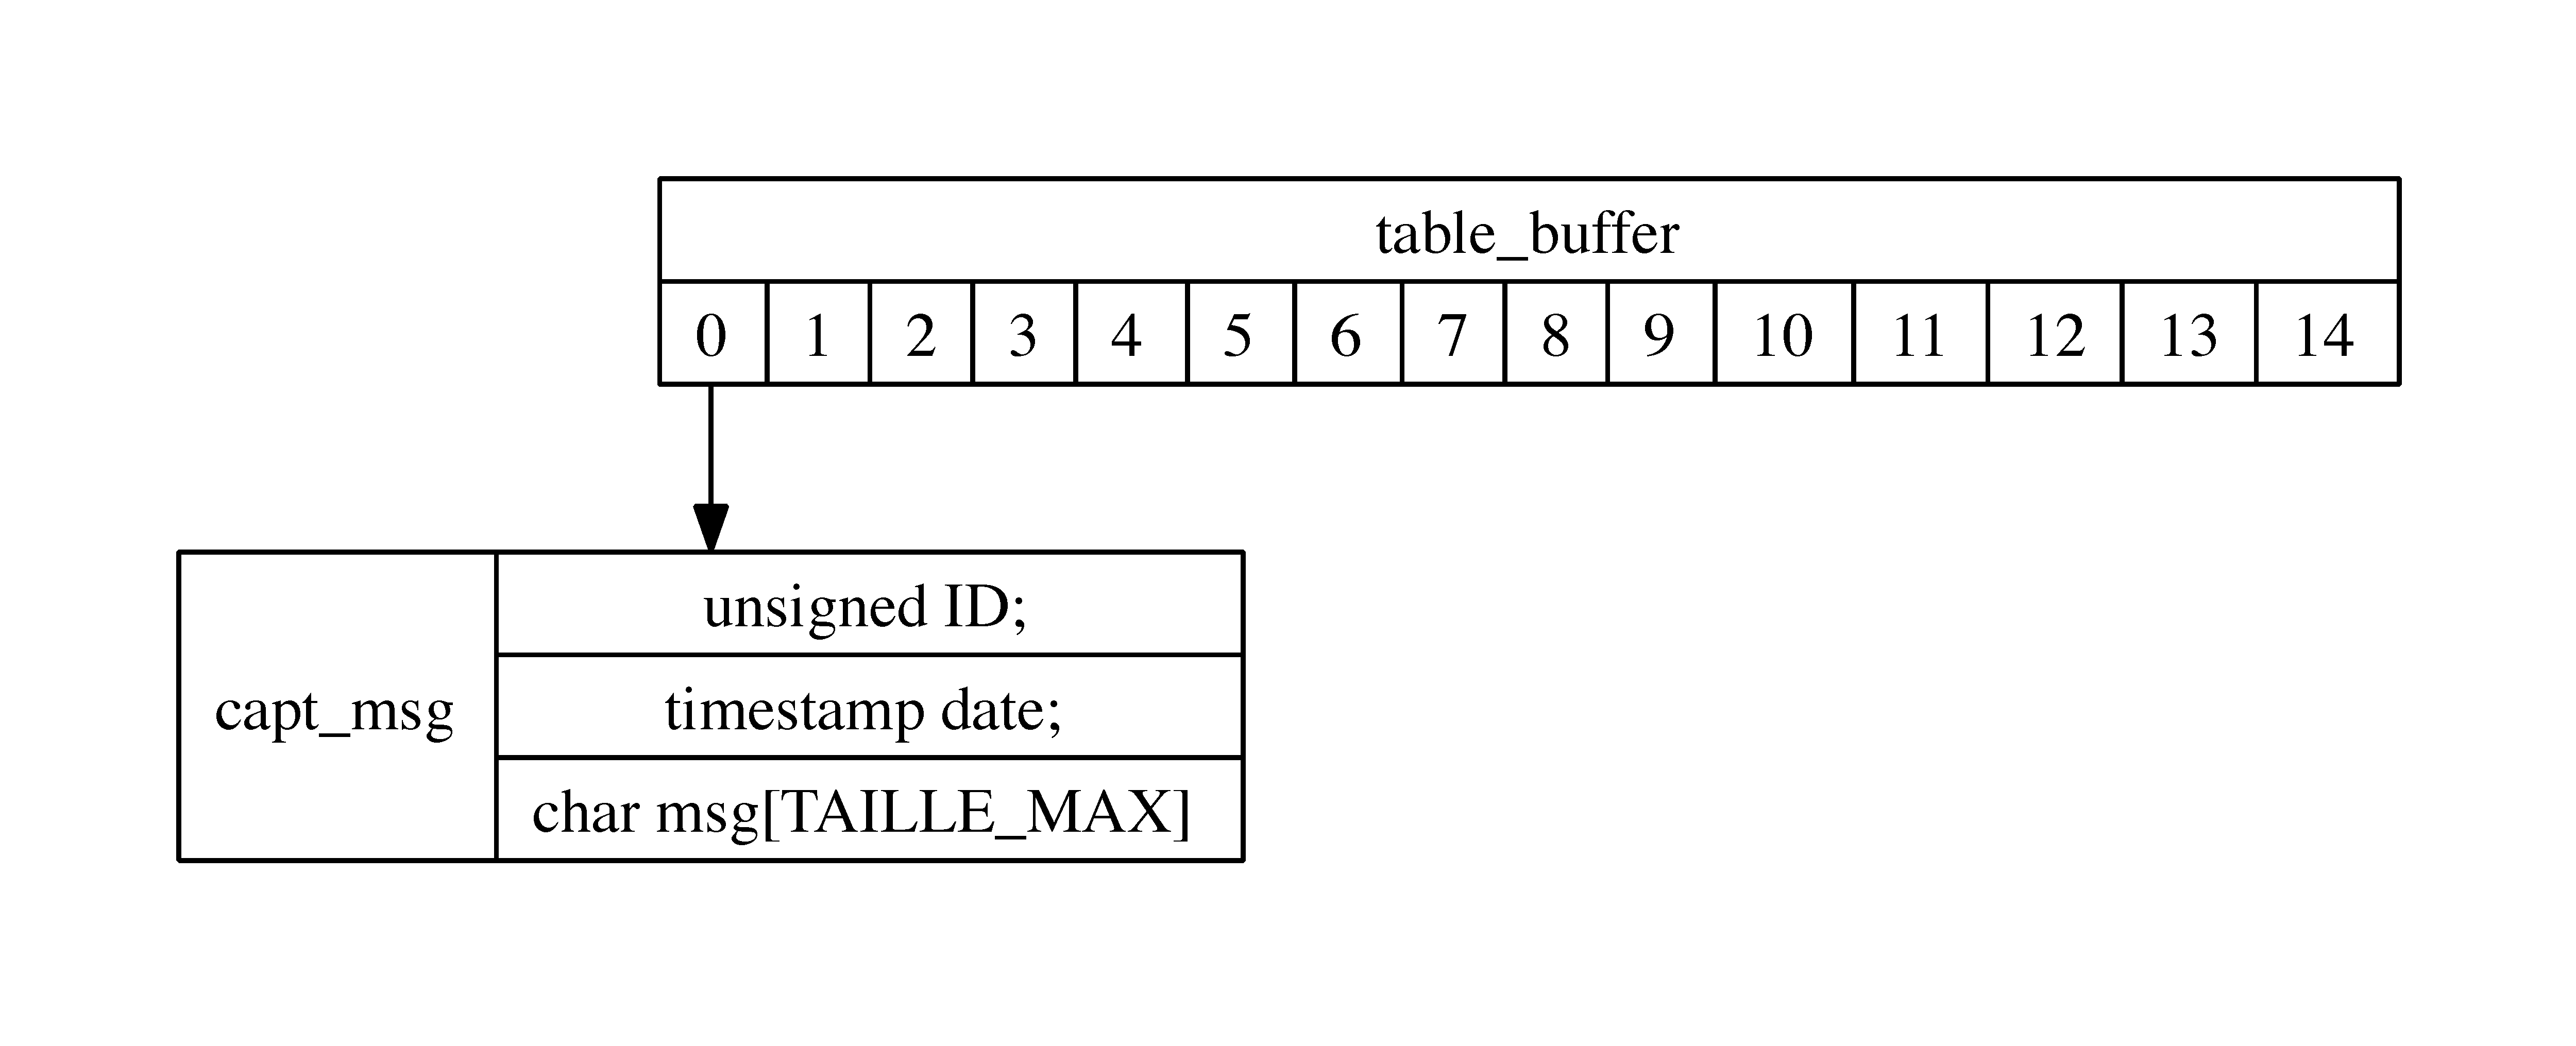
\includegraphics[width=\textwidth]{ressources/table_buffer.pdf}\\

\section{Conception graphique}

\subsection{\kw{pe\_driverInstall}}
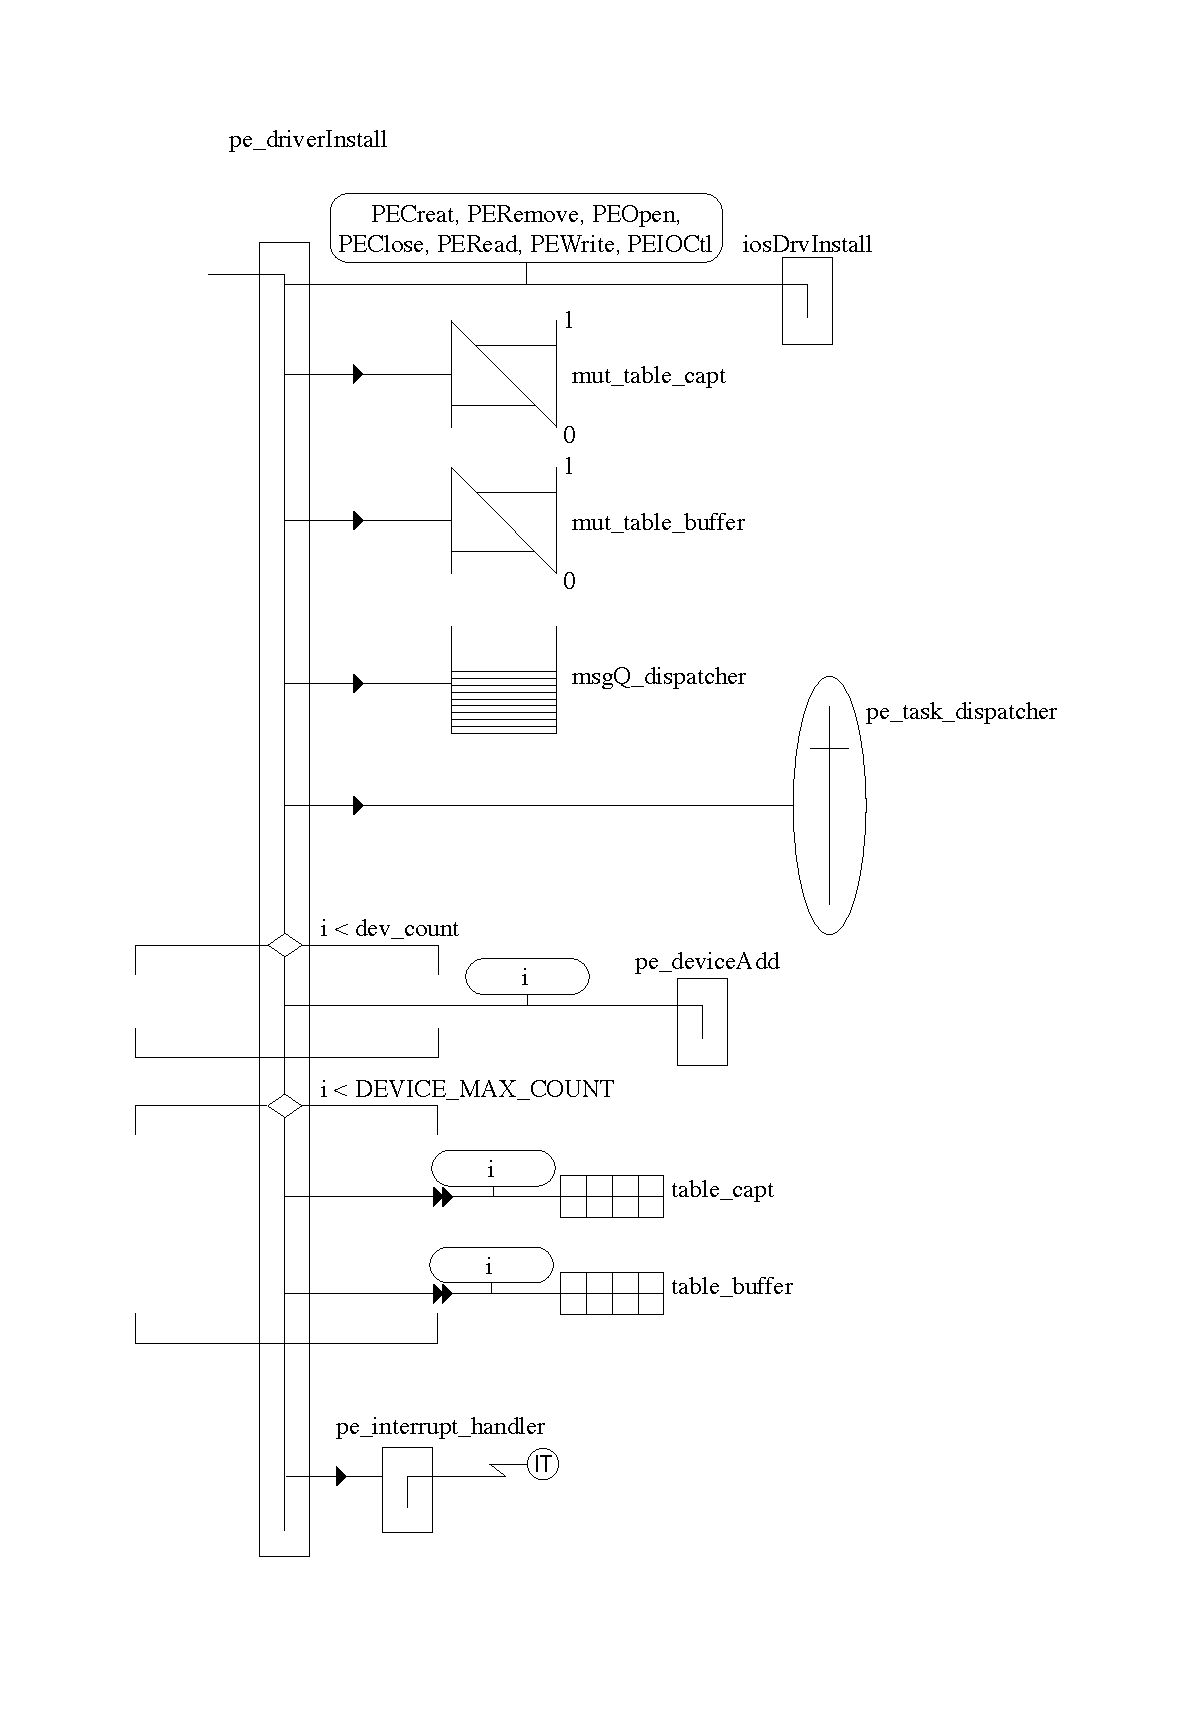
\includegraphics[width=\textwidth]{ressources/pe_driverInstall.pdf}
\subsection{\kw{pe\_driverUnInstall}}
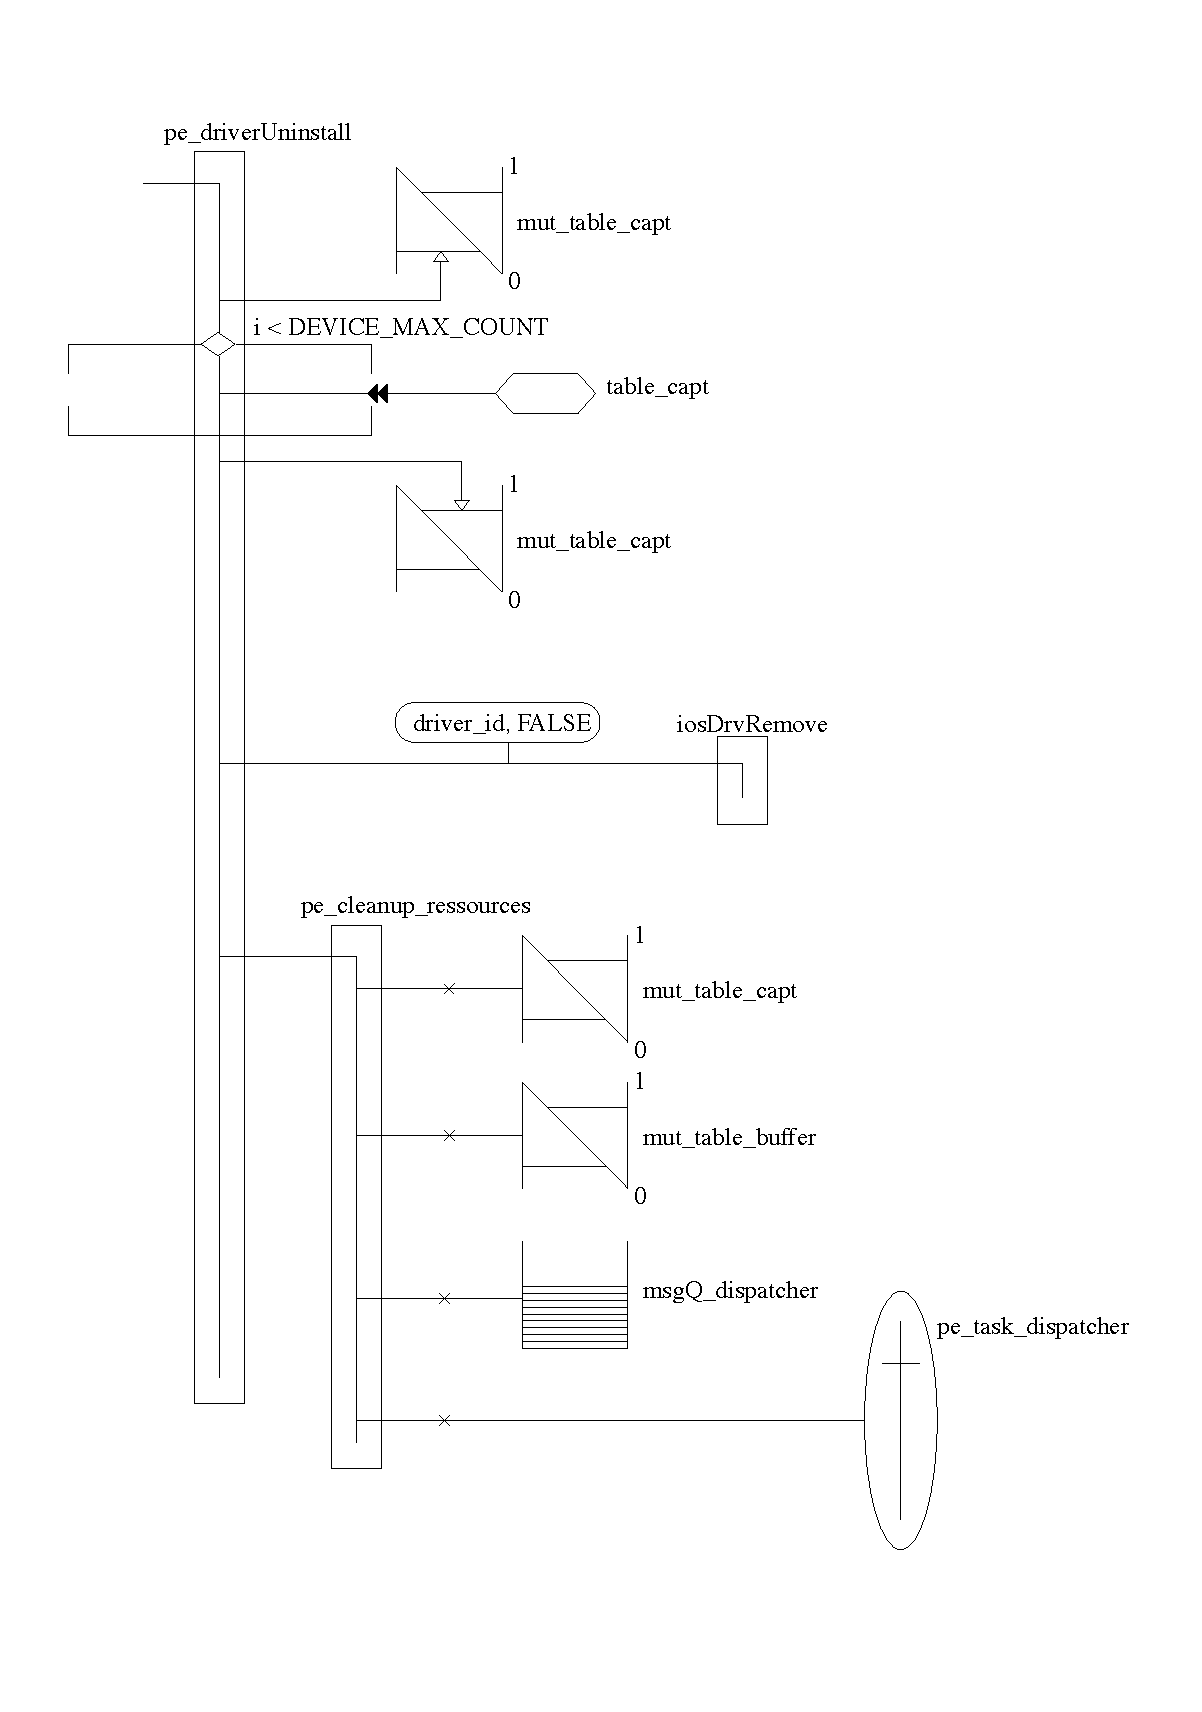
\includegraphics[width=\textwidth]{ressources/pe_driverUninstall.pdf}
\subsection{\kw{pe\_deviceAdd}}
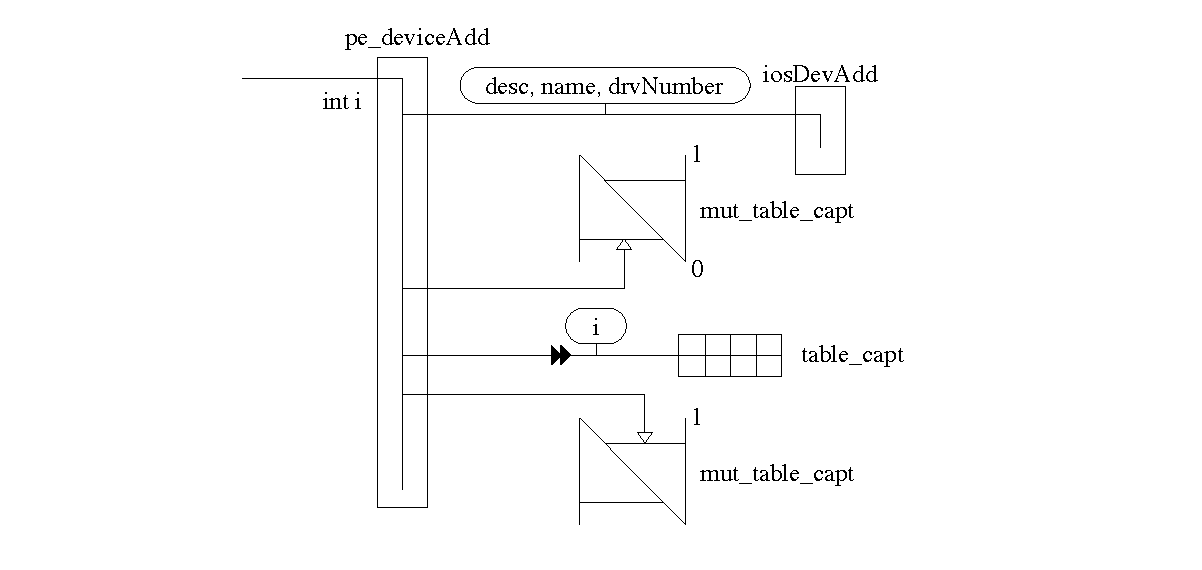
\includegraphics[width=\textwidth]{ressources/pe_deviceAdd.pdf}
\subsection{\kw{pe\_deviceRemove}}
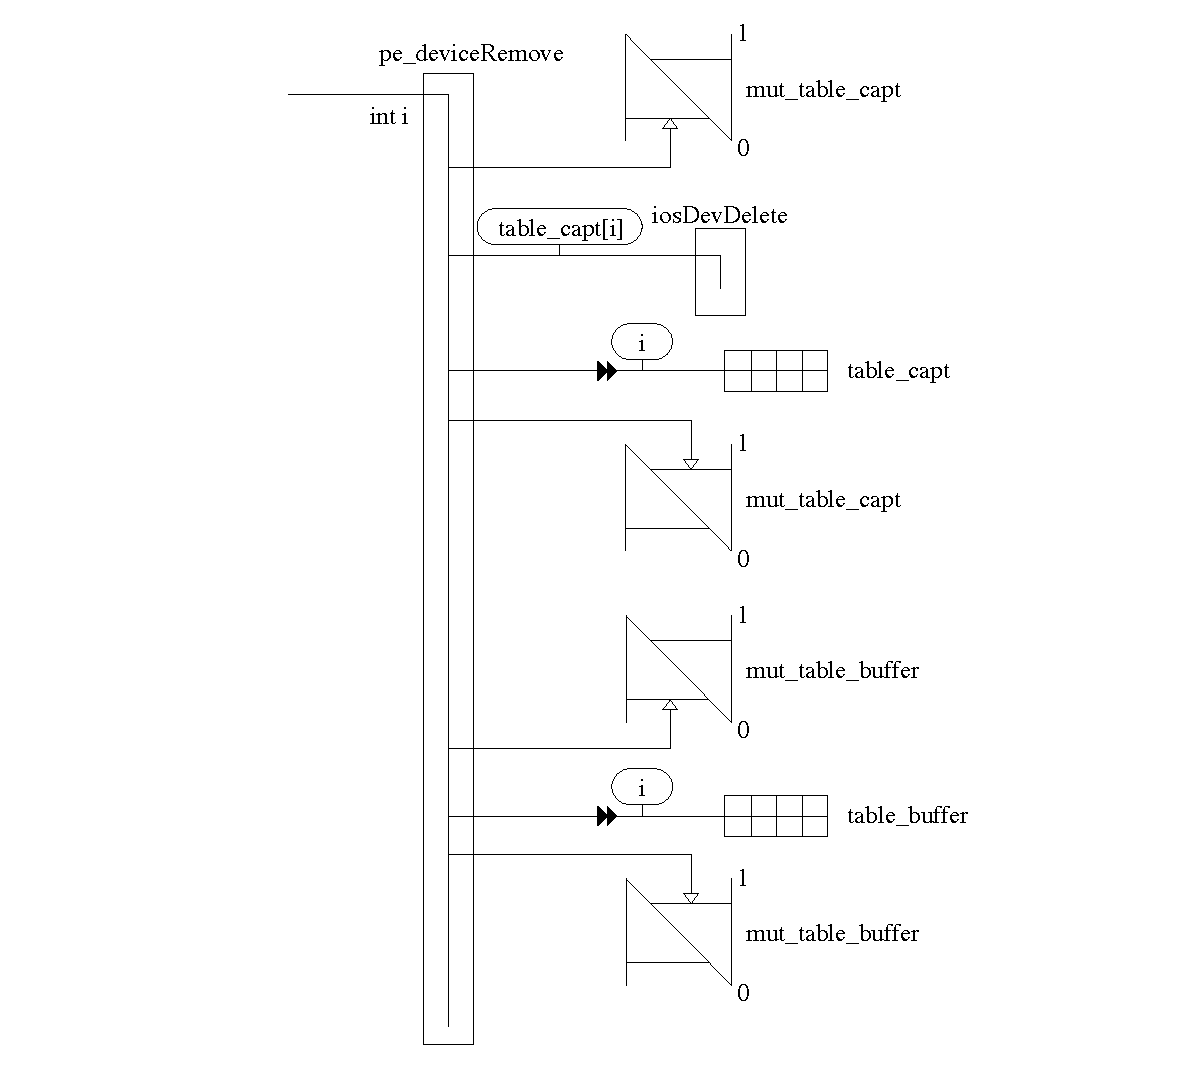
\includegraphics[width=\textwidth]{ressources/pe_deviceRemove.pdf}
\subsection{\kw{Interrut\_handler}}
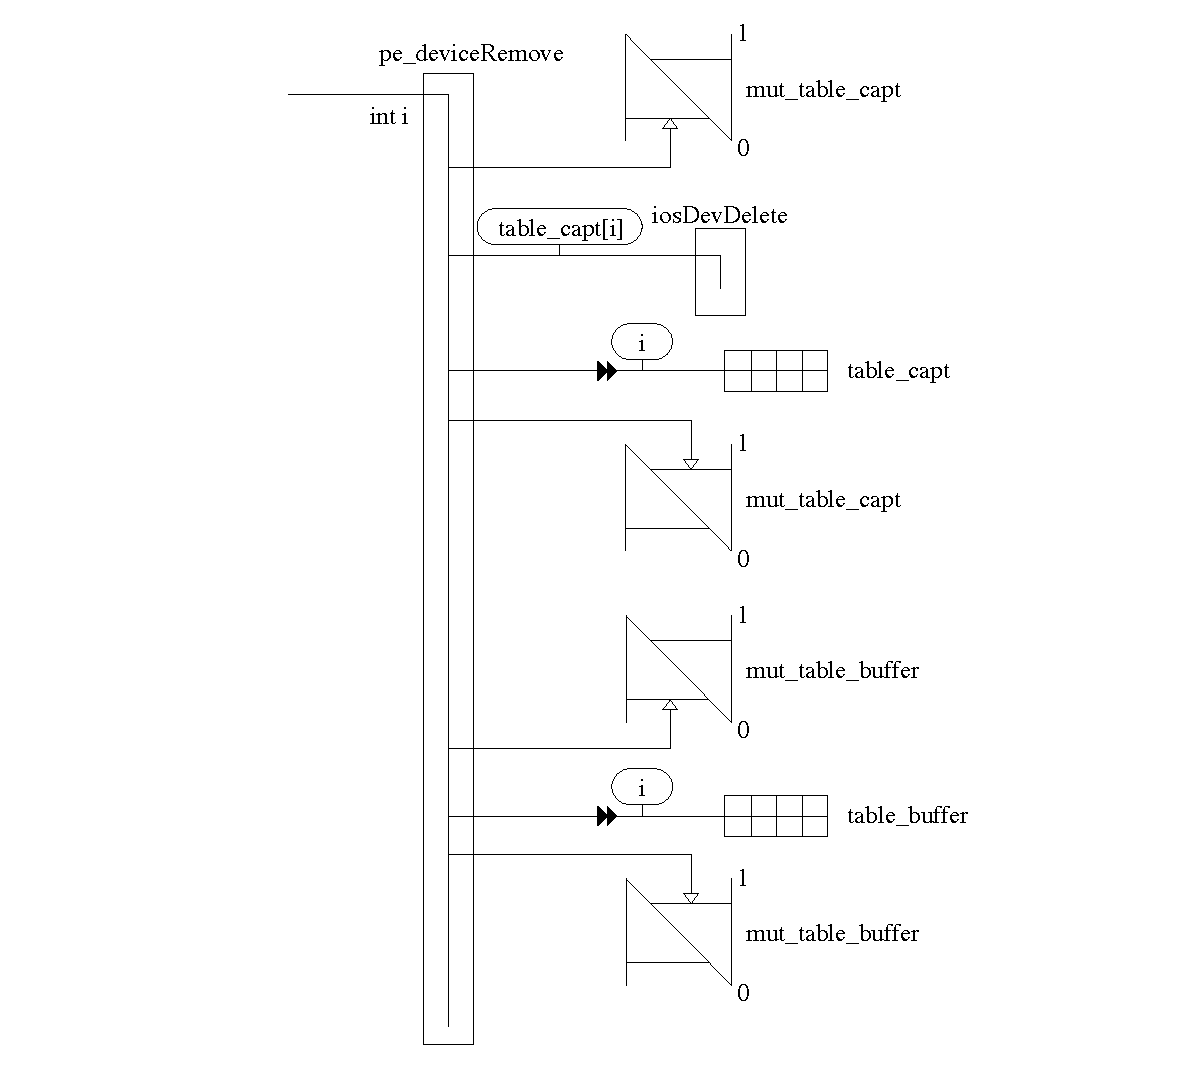
\includegraphics[width=\textwidth]{ressources/pe_deviceRemove.pdf}
\subsection{\kw{pe\_task\_dispatcher}}
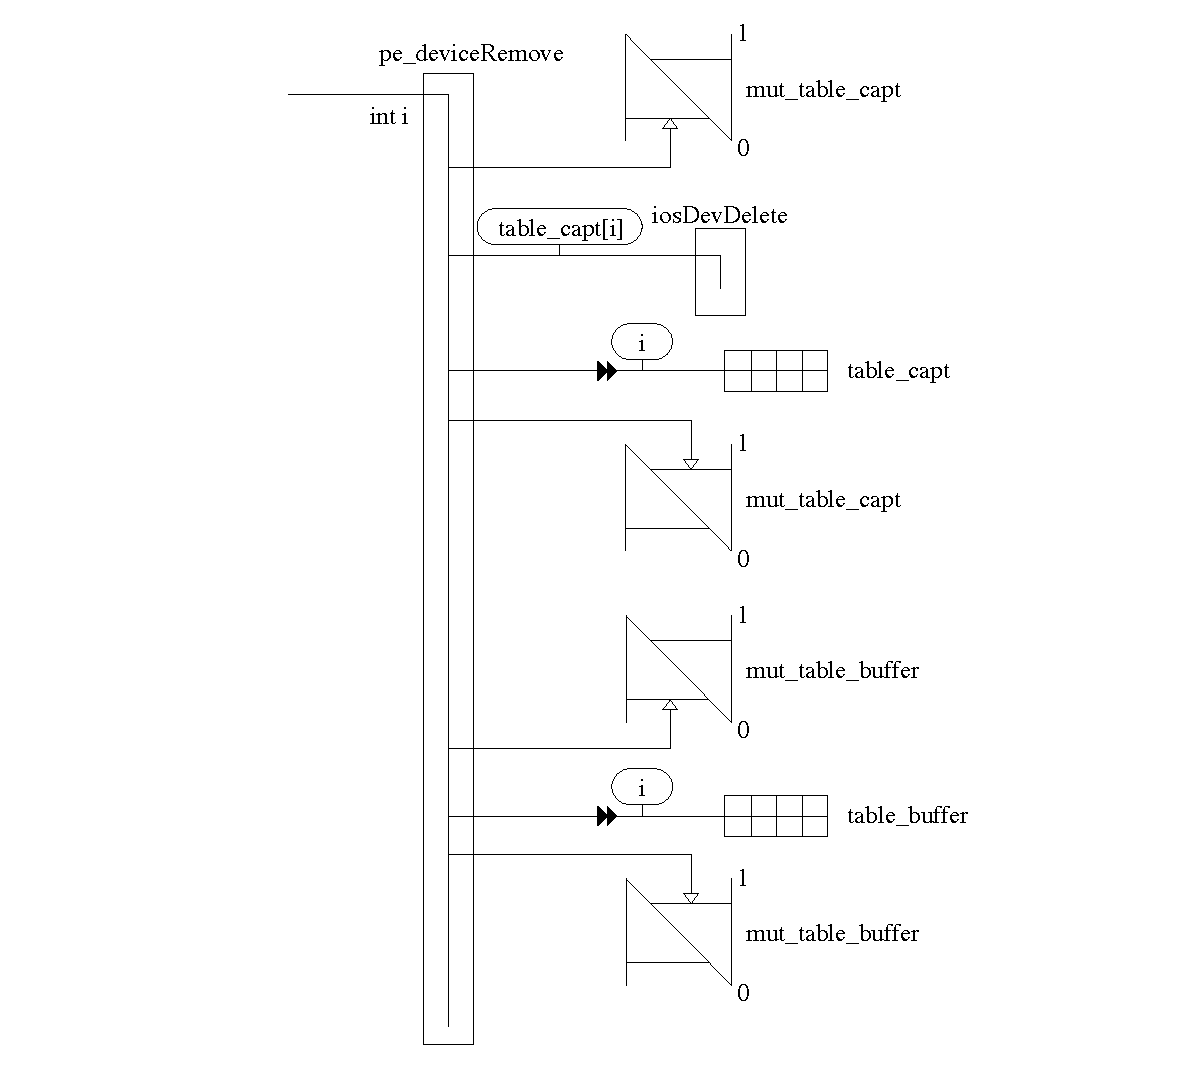
\includegraphics[width=\textwidth]{ressources/pe_deviceRemove.pdf}
\subsection{\kw{pe\_open}}
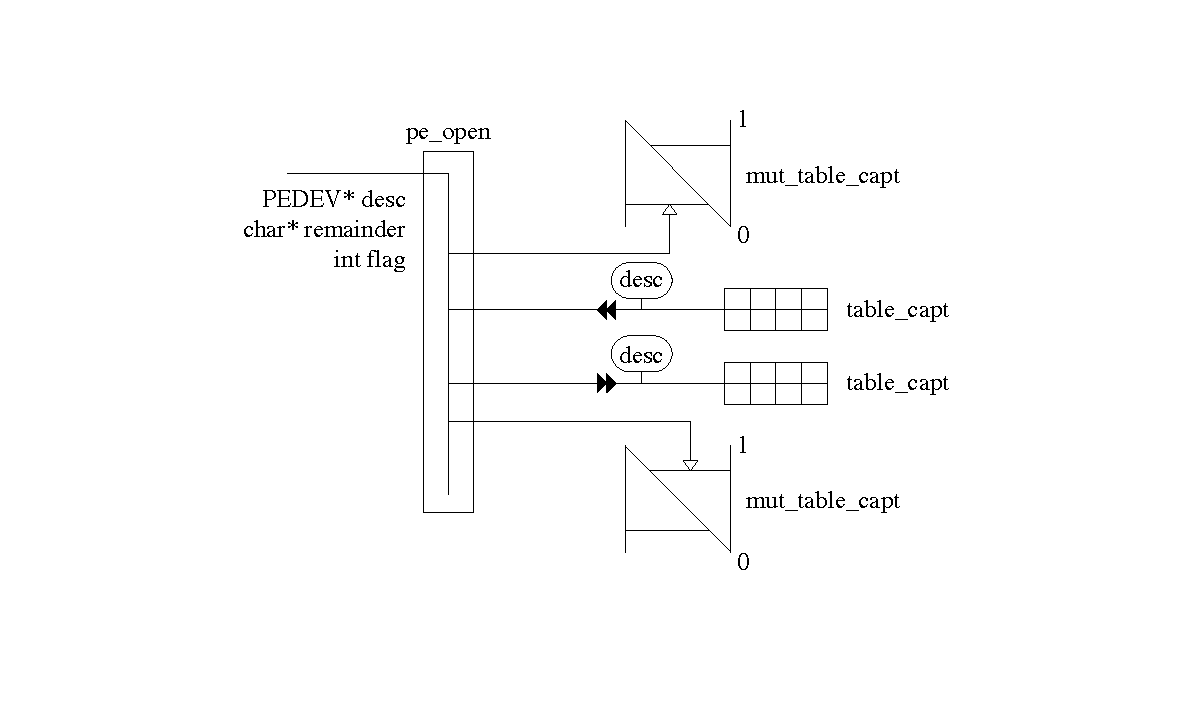
\includegraphics[width=\textwidth]{ressources/pe_open.pdf}
\subsection{\kw{pe\_read}}
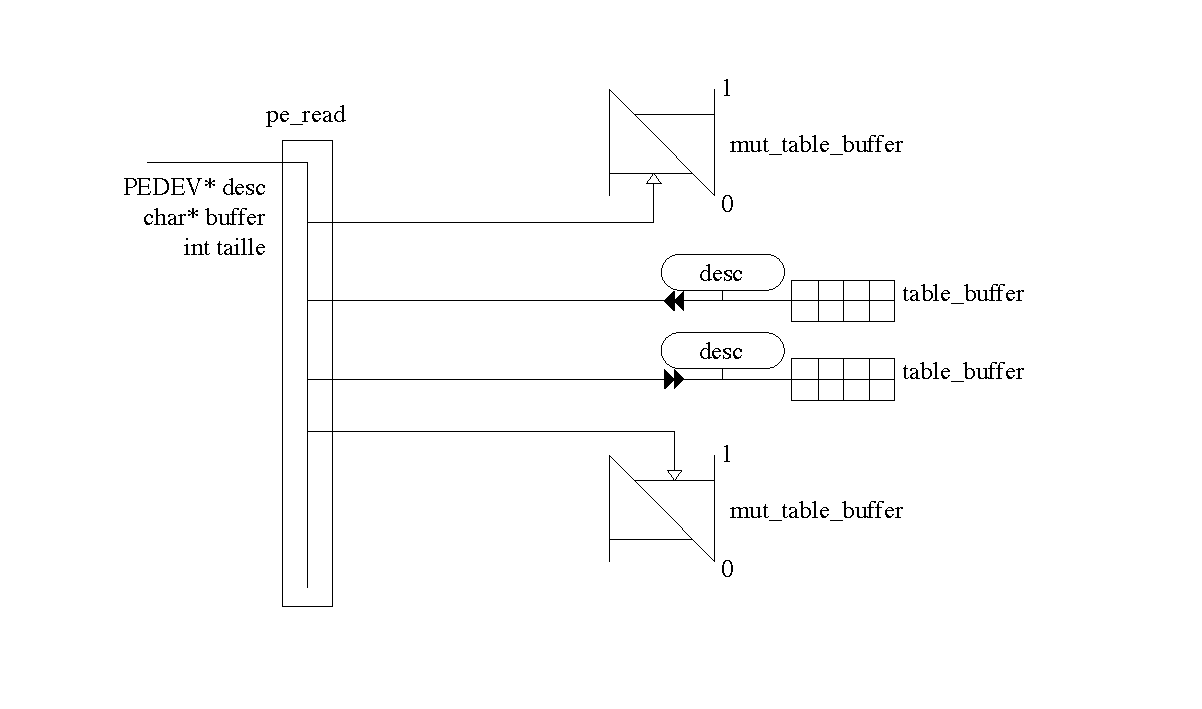
\includegraphics[width=\textwidth]{ressources/pe_read.pdf}
\subsection{\kw{pe\_close}}
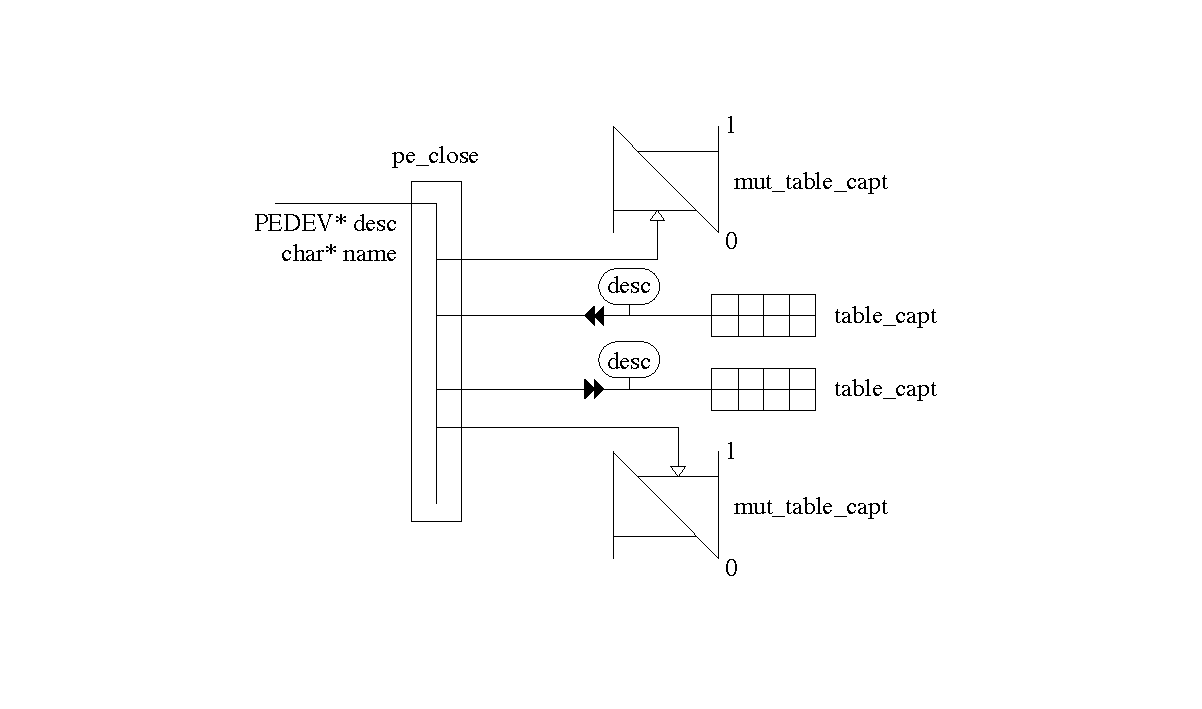
\includegraphics[width=\textwidth]{ressources/pe_close.pdf}
\subsection{\kw{pe\_ioctl}}
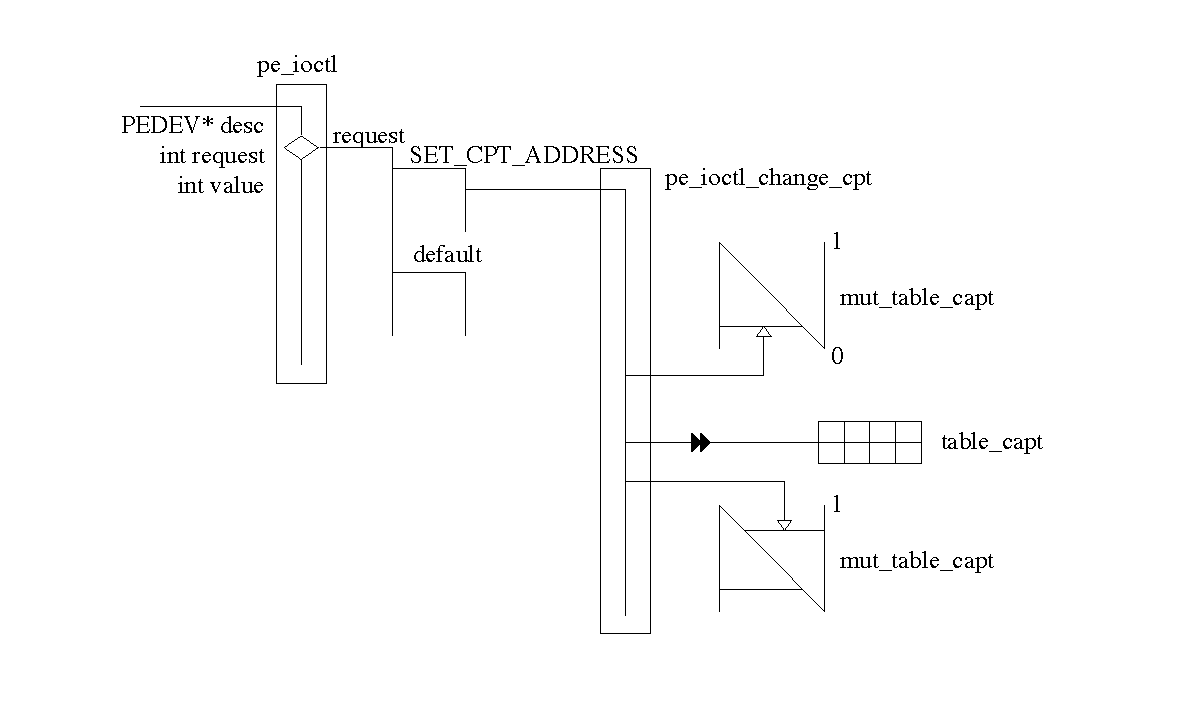
\includegraphics[width=\textwidth]{ressources/pe_ioctl.pdf}

\newpage
\section{Plan de test}
\Test{Installation d'un driver}
{Installer le driver alors qu'il n'est pas installé}
{La valeur de retour doit être positive, et correspond au numéro du driver. Il
doit être possible de le retrouver en utilisant la fonction \kw{iosDrvShow}.}

\Test{Installation d'un driver déjà installé}
{Installer le driver alors qu'il est déjà installé : appeler deux fois \kw{iosDrvInstall}.}
{La première installation doit bien se passer (valeur de retour positive).  Le second appel de \kw{iosDrvInstall} doit renvoyer \kw{ERROR}.}

\Test{Retrait d'un driver}
{Utilisation de la fonction \kw{iosDrvRemove}, alors que le pilote est installé sur le système, et qu'il n'est pas utilisé.}
{La valeur de retour doit être égale à \kw{OK}.}

\Test{Retrait du driver alors qu'il n'est pas installé}
{Utilisation de la fonction \kw{iosDrvRemove}, alors que le pilote n'est pas
installé sur le système.}
{La valeur de retour doit être \kw{ERROR}.}

\Test{Retrait du driver alors qu'un périphérique est ouvert}
{Alors qu'un capteur a été ouvert en lecture, retirer le driver, à l'aide de la
fonction \kw{iosDrvRemove}.}
{La fonction doit retourner \kw{ERROR}, et \kw{errno} doit être
    positionné à \kw{ECPTBUSY}. Le driver ne doit pas être retiré.}

\Test{Ajout d'un périphérique}
{Utilisation de la fonction \kw{iosDevAdd}, une seule fois, avec des paramètre valides.}
{La valeur de retour doit être \kw{OK}, le périphérique doit être trouvable en utilisant \kw{iosDevFind}, qui ne doit pas renvoyer \kw{NULL}.}

\Test{Retrait d'un périphérique}
{Utilisation de la fonction \kw{iosDevDelete}, avec des paramètres valides.}
{Il ne doit plus être possible d'ouvrir le périphérique : un appel à \kw{open}
sur ce périphérique doit échouer (il doit retourner \kw{ERROR}), et \kw{errno}
doit être positionné à \kw{ENEXIST}.}

\Test{Ajout d'un périphérique alors que 15 périphériques ont été ajoutés.}
{Utilisation de la fonction \kw{iosDevAdd}, 16 fois, avec des paramètres valides.}
{Le 16\ieme~appel à \kw{iosDevAdd} doit provoquer une erreur, et renvoyer \kw{ERROR}.}

\Test{Ouverture d'un capteur}
{Appeler \kw{open} sur un capteur valide (le fichier existe et est accessible en écriture), avec des options valide (\kw{O\_RDONLY}), une seule fois.} 
{La valeur de retour doit être un entier positif.}~

\Test{Ouverture d'un capteur déjà ouvert}
{Appeler \kw{open} sur un capteur valide (le fichier existe, et est accessible
	en lecture), alors qu'il vient d'être ouvert avec succès.}
{\kw{open} doit renvoyer \kw{ERROR}, et \kw{errno} doit être positionné à \kw{EALREADYOPENED}.}

\Test{Ouverture d'un capteur avec des paramètres invalides}
{Appeler \kw{open} sur un capteur valide (le fichier existe, et est accessible
en lecture/écriture, en passant un \kw{mode} différent de \kw{O\_RDONLY}.}.
{L'appel doit échouer, et donc renvoyer \kw{ERROR}. De plus, \kw{errno} doit
être positionné à \kw{EARG}.}

\Test{Fermeture d'un capteur}
{Appeler \kw{close} sur un descripteur de fichier valide (qui a été ouvert avec
succès précédemment), et qui n'a pas été fermé depuis.}
{La valeur de retour doit être égale à \kw{OK}}

\Test{Lecture d'une valeur dans un capteur}
{Utiliser \kw{read} sur un capteur ouvert avec succès}
{La valeur de retour doit être un nombre positif, et doit être cohérente par
    rapport aux paramètre d'appel de \kw{read}.}

\Test{Utilisation de \kw{read} avec une taille de lecture invalide}
{Utilisation de l'appel système \kw{read} avec une descripteur de fichier
    valide, mais avec une taille de lecture négative.}
{L'appel doit échouer en renvoyant -1, et \kw{errno} doit être positionné à
    \kw{EARG}.}

\Test{Utilisation de \kw{ioctl} avec des paramètres corrects}
{Utilisation de \kw{ioctl} avec des paramètres corrects : un descripteur de
fichier valide, une valeur pour \kw{request} égale à la constante
\kw{CHANGEMENT\_CAPTEUR}, et une valeur pour \kw{value} inférieur ou égale
à 255, correspondant bien à un capteur valide.}
{La valeur de retour doit être égale à \kw{OK}, ou alors elle doit être égale
à \kw{ERROR}, mais alors \kw{errno} doit être positionné à \kw{ECPTBUSY}, et
le même appel effectué ultérieurement doit renvoyer \kw{OK}.}

\Test{Utilisation de \kw{ioctl} avec de mauvais arguments}
{Utilisation de la fonction \kw{ioctl} avec un second paramètre correspondant à
une fonction non-implémenté. Le descripteur de fichier passé en tant que premier
paramètre doit être valide, et correspondre à un périphérique géré par le
driver.}
{L'appel doit échouer (la valeur de retour doit être égale à \kw{ERROR}), et
    \kw{errno} doit être positionné à \kw{EARG}.}

\Test{Utilisation de \kw{ioctl} pour associer le même capteur à deux
    descripteur de fichiers}
{On utilise la fonction \kw{ioctl} deux fois, avec des descripteurs de fichier
    différents, mais avec le même numéro de capteur.}
{L'appel doit échouer, et renvoyer \kw{ERROR}. \kw{errno} doit alors être
positionné à \kw{EARG}.}

\Test{Utilisation de \kw{write}}
{Appel de write sur un capteur ouvert avec succès.}
{L'appel doit échouer, et \kw{errno} doit être positionné à \kw{ENOTSUP}.}

\Test{Retrait d'un périphérique ouvert}
{Tentative de retrait d'un périphérique sur lequel un appel de \kw{open} a été
    effectué avec succès précédemment, et sur lequel on n'a pas fait d'appel à
	\kw{close} ou \kw{remove}.}
{L'appel doit réussir : la valeur de retour doit être égale à \kw{OK}.}

\Test{Retrait d'un périphérique qui n'existe pas}
{Tentative de retrait d'un périphérique qui n'existe pas.}
{L'appel doit échouer, et retourner \kw{ERROR}. \kw{errno} doit être positionné
    à \kw{ENEXIST}.}


\end{document}
